\section{Expériences}
    \subsection{Introduction}
    Dans ce chapitre, nous allons définir et aborder toutes les notions théoriques nécessaires
    pour chaque expérience, ainsi que les valeurs expérimentales mesurées et la discussion des résultats.

    \subsection{Détermination de la constante de raideur du ressort}
        \subsubsection{Objectif}
            L'objectif de cette expérience est de déterminer la constante de raideur de trois ressorts
            en utilisant la méthode de la régression linéaire.
        \subsubsection{schéma du système}
            Nous allons étudier un système composé d'un ressort, de plusieurs masses et d'un capteur CASSY.
            \begin{figure}[h]
    \centering
    \begin{tikzpicture}
        % Equilibrium Position
        % Ground and frame
        \draw[thick] (-1,5) -- (1,5); % Top bar
        \draw[thick] (-1,5) -- (-1,0); % Side bar
        
        % Sensor
        \draw[fill, pattern=north east lines] (0.5,5) rectangle (1,5.5);
        
        % Laser
        \draw[red, thick] (0.75,5) -- (0.75,3.3); % Laser stopping at plate
        
        % Vertical x-axis with cut line (on the left)
        \node[below, blue] at (-1.2,0) {$x$};
        \draw[blue, thick, ->] (-1.2,5) -- (-1.2,0);
        \node[left, blue] at (-1.2,3.31) {$0$};
        \draw[blue, thick] (-1.25,3.31) -- (-1.15,3.31); % Cut mark for 0
        \draw[blue, thin] (-1.2,3.308) -- (-0.8,3.308); % Cut line from x-axis to plate
        
        % Spring (equilibrium position, more loops)
        \draw[decorate, decoration={coil,aspect=0.7,segment length=3.5mm,amplitude=3mm}] (0,5) -- (0,3.4);
        \draw[thin] (0,3.4) -- (0,3.3); % Extended bottom vertical line
        
        % Thin plate attached to the spring (longer and fully above mass)
        \draw[thick] (-0.8,3.3) rectangle (0.8,3.2); % Longer rectangle plate

    \end{tikzpicture}
    \hspace{1cm}
    \begin{tikzpicture}
        % Elongated Position
        % Ground and frame
        \draw[thick] (-1,5) -- (1,5); % Top bar
        \draw[thick] (-1,5) -- (-1,0); % Side bar
        
        % Sensor
        \draw[fill, pattern=north east lines] (0.5,5) rectangle (1,5.5);
        
        % Laser
        \draw[red, thick] (0.75,5) -- (0.75,1.8); % Laser stopping at plate
        
        % Vertical x-axis with cut line (on the left)
        \node[below, blue] at (-1.2,0) {$x$};
        \draw[blue, thick, ->] (-1.2,5) -- (-1.2,0);
        \node[left, blue] at (-1.2,1.8) {$x_1$};
        \draw[blue, thick] (-1.25,1.81) -- (-1.15,1.81); % Cut mark for X1
        \draw[blue, thin] (-1.2,1.81) -- (0,1.8); % Cut line from x-axis to plate
        
        % Spring (elongated position, more spaced loops, extended bottom part)
        \draw[decorate, decoration={coil,aspect=0.7,segment length=5mm,amplitude=3mm}] (0,5) -- (0,2.2);
        \draw[thick] (0,2.2) -- (0,1.8); % Extended bottom vertical line
        
        % Thin plate attached to the spring (longer and fully above mass)
        \draw[thick] (-0.8,1.8) rectangle (0.8,1.7); % Longer rectangle plate
        
        % Mass (elongated position, moved lower)
        \draw[thick] (-0.5,1.5) rectangle (0.5,1.0);
        \node at (0,1.25) {$m_s$};
        
        % Gravity
        \draw[->, teal, thick] (0,1.0) -- (0,0.3);
        \node[right, teal] at (0,0.2) {$m_s \vec{g}$};
        
        % Spring force
        \draw[->, teal, thick] (0,1.5) -- (0,2.3);
        \node[left, teal] at (0,2.3) {$\vec{F_r}$};
    \end{tikzpicture}
    \caption{Position au repos et position allongée du système à l'équilibre.}
\end{figure}
\FloatBarrier
            Nous pouvons voir à la figure 1 le schéma du système que nous allons étudier. On 
            utilise un plateau permettant de refléter le laser partant du capteur CASSY.
            Nous le calibrons pour qu'il soit à l'origine du repère, puis nous laissons
            tomber le ressort avec la surcharge jusqu'à sa position d'équilibre.
            Nous pouvons donc utiliser la seconde loi de Newton pour déterminer théoriquement
            la constante de raideur du ressort : 
            \begin{equation}
                \sum \vec{F}_{ext} = m \vec{a}
            \end{equation}
            Dans le cas où le ressort est à l'équilibre, nous avons :
            \begin{equation}
                \sum \vec{F}_{ext} = \vec{0}
            \end{equation}
            Nous pouvons écrire la somme des forces comme suit :
            \begin{equation}
                \vec{F_r} + m_s\vec{g} = \vec{0}
            \end{equation}
            \begin{align*}
                \Leftrightarrow & -k\Delta x \vec{e_x} + m_s g \vec{e_x} = 0 \\
                \Leftrightarrow & \quad m_s g = k \Delta x \\
                \Leftrightarrow & \quad k = \frac{m_s g}{\Delta x} \\
                \Leftrightarrow & \quad k = \frac{m_s g}{x_1 - x_0}
            \end{align*}
            Nous avons que $x_0 = 0$, alors nous pouvons écrire :
            \begin{equation}
                k = \frac{m_s g}{x_1}
            \end{equation}
            Ou encore, nous pouvons (et nous allons) déterminer graphiquement la constante
            de raideur du ressort. Pour ceci, nous allons utiliser la pente de la droite obtenue
            par la régression linéaire des points de la force en fonction de la position trouvée
            expérimentalement. Nous avons donc :
            \begin{equation}
                k = \frac{\Delta F_p}{\Delta x}
            \end{equation}
            Où $\Delta F_p$ est la différence entre les forces maximale et minimale,
            et $\Delta x$ est la différence entre les positions maximale et minimale.
            \newline
            Nous avons donc tout ce qu'il nous faut pour déterminer la constante de raideur
            du ressort.

            \newpage

        \subsubsection{valeurs expérimentales}
            Nous avons effectué l'expérience avec trois ressorts différents et cinq surcharges
            différentes pour chaque ressort. Nous avons mesuré les positions des ressorts à l'équilibre, ainsi que
            les forces correspondantes. Nous avons obtenu les valeurs suivantes :
            \begin{figure}[h]
                \centering
                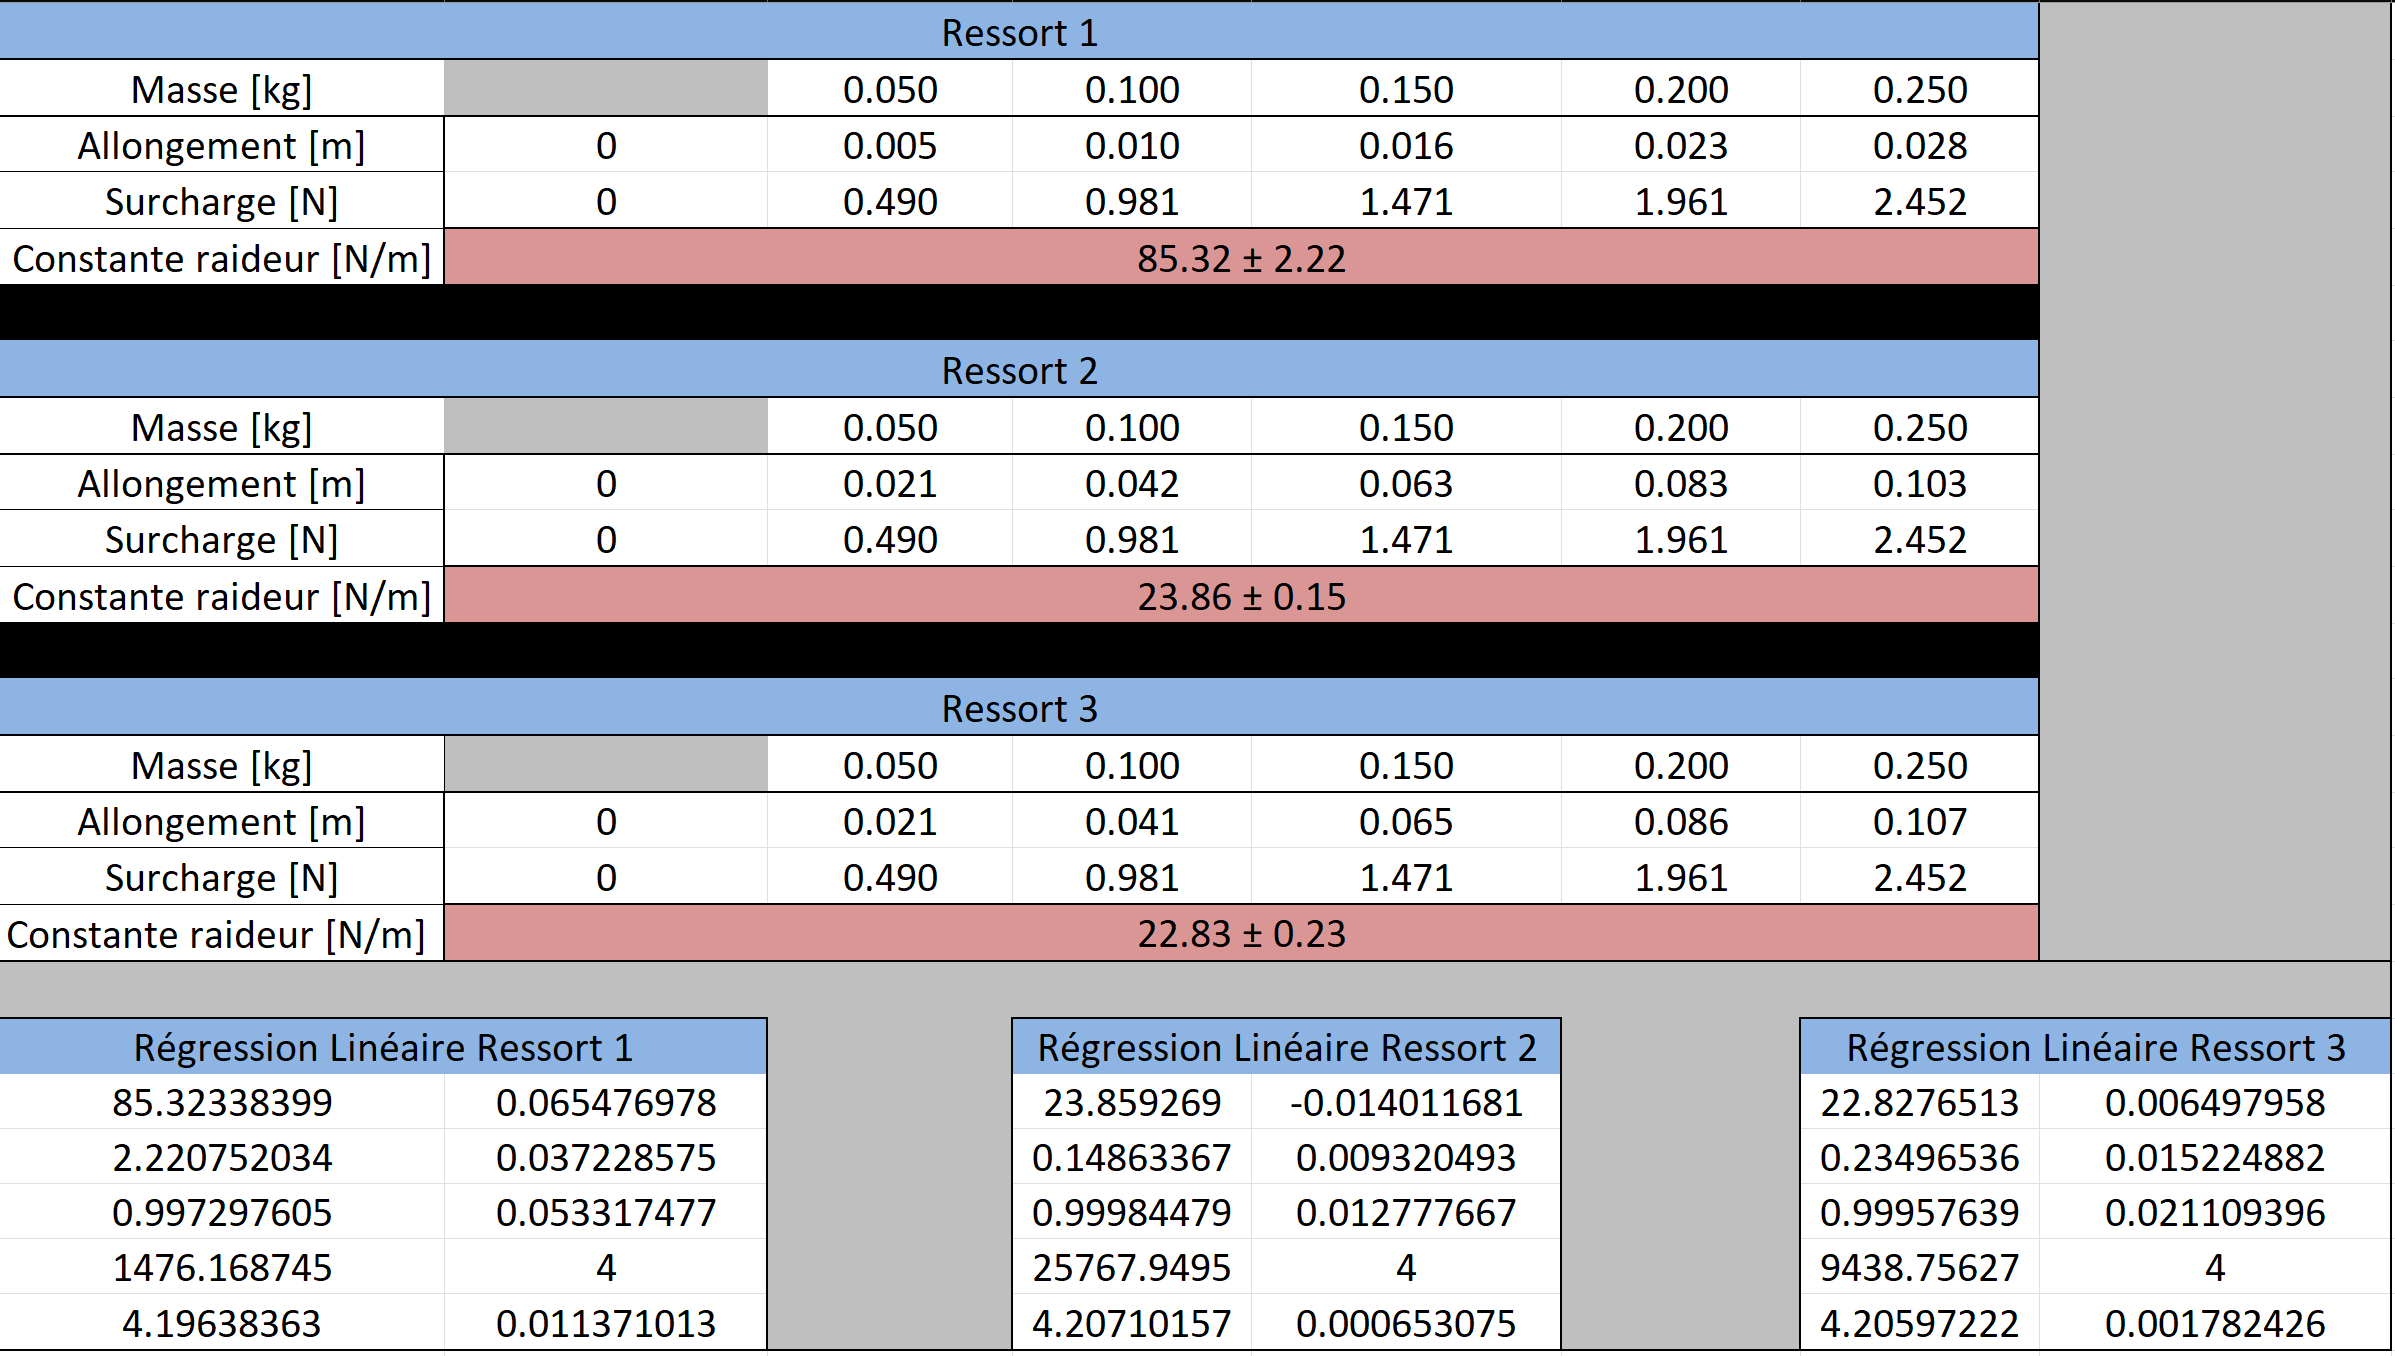
\includegraphics[width=0.69\textwidth]{images/Capture.PNG}
                \caption{Valeurs expérimentales de la force en fonction de la position des ressorts}
            \end{figure}
            \hspace{1cm}
            \begin{figure}[h]
                \centering
                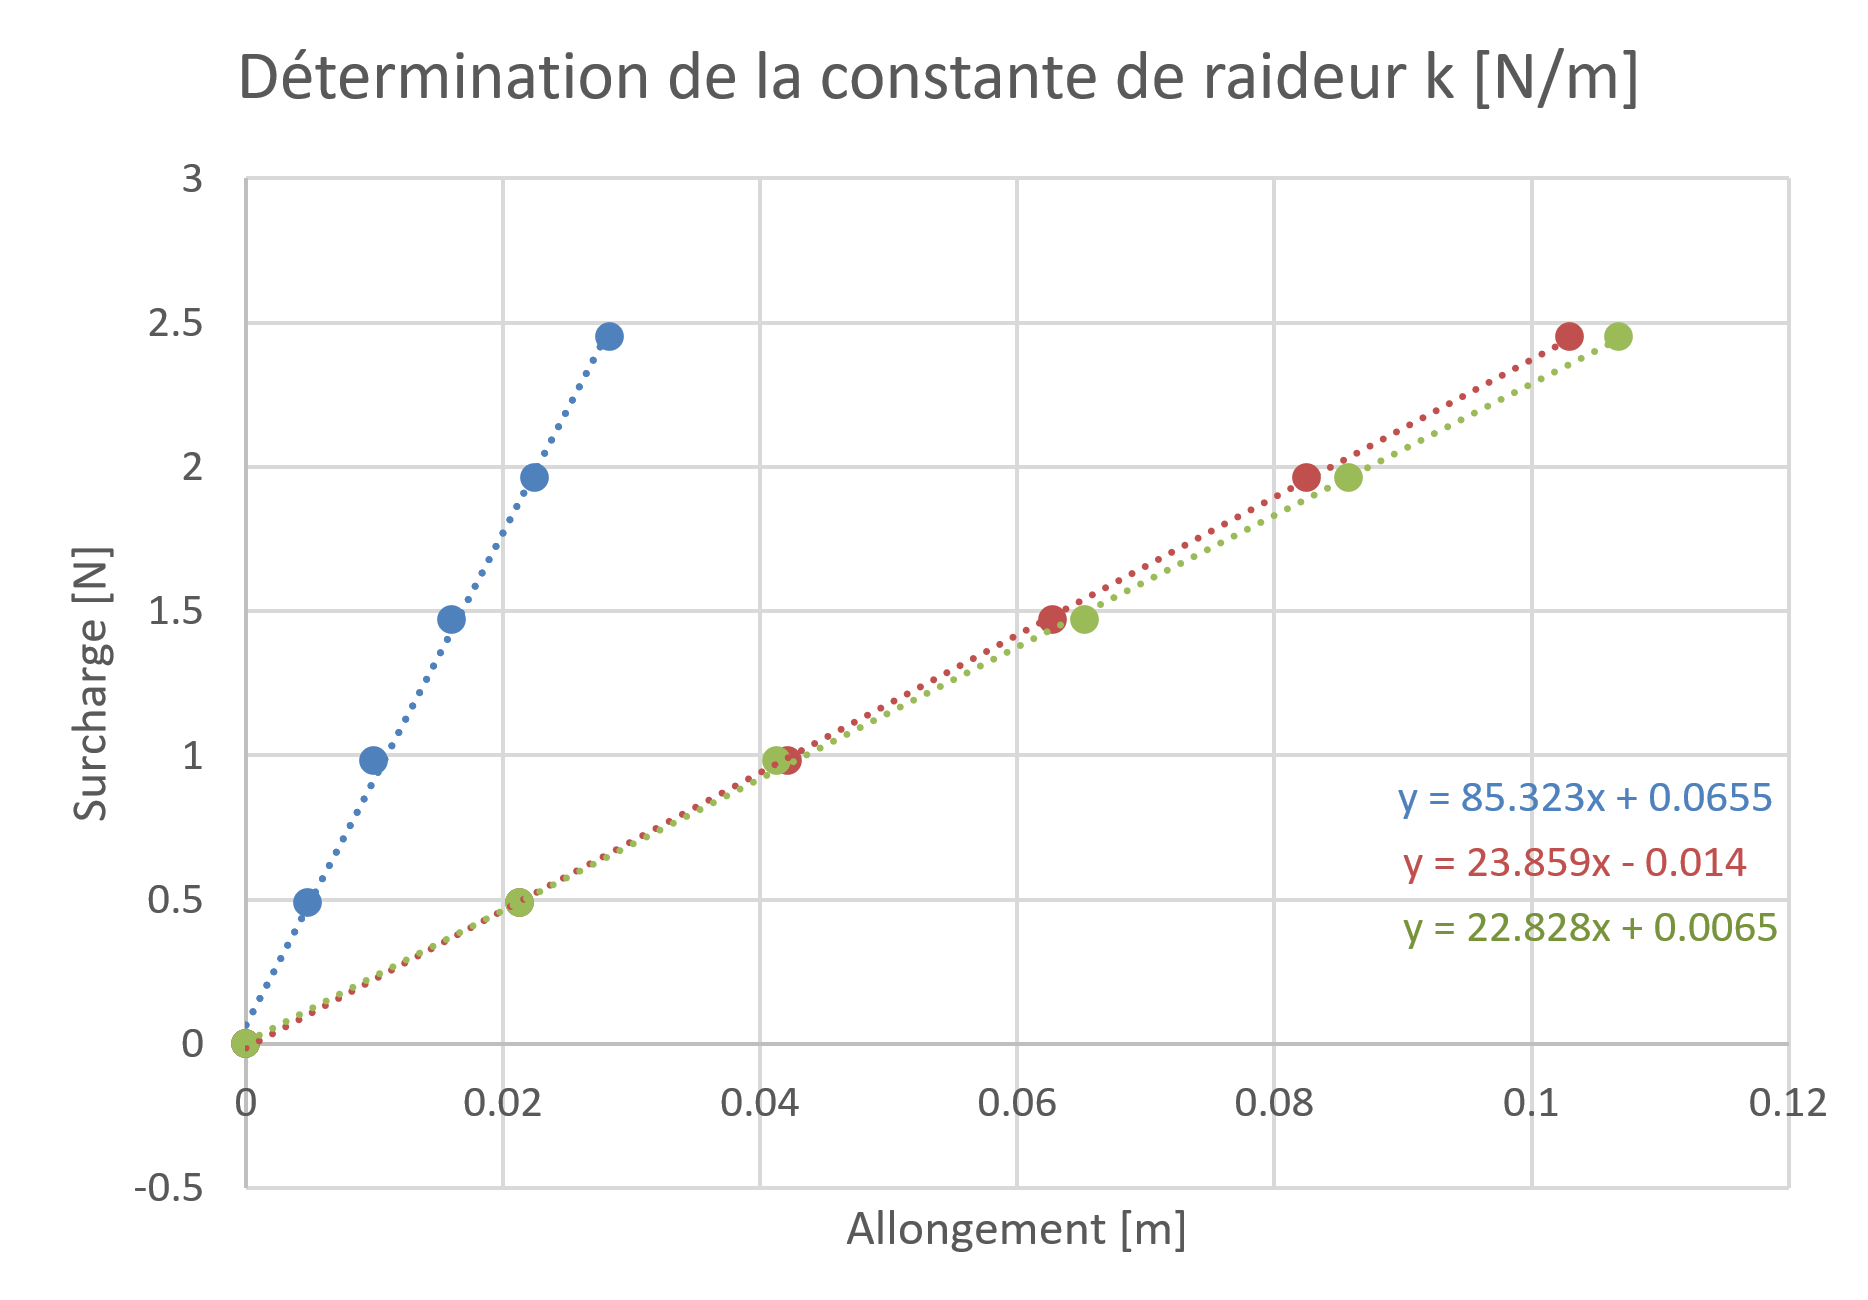
\includegraphics[width=0.6\textwidth]{images/graphe_k.PNG}
                \caption{Graphe de la force en fonction de la position des ressorts}
            \end{figure}

            \newpage

            \begin{figure}[h]
                \centering
                \begin{minipage}{0.31\textwidth}
                    \centering
                    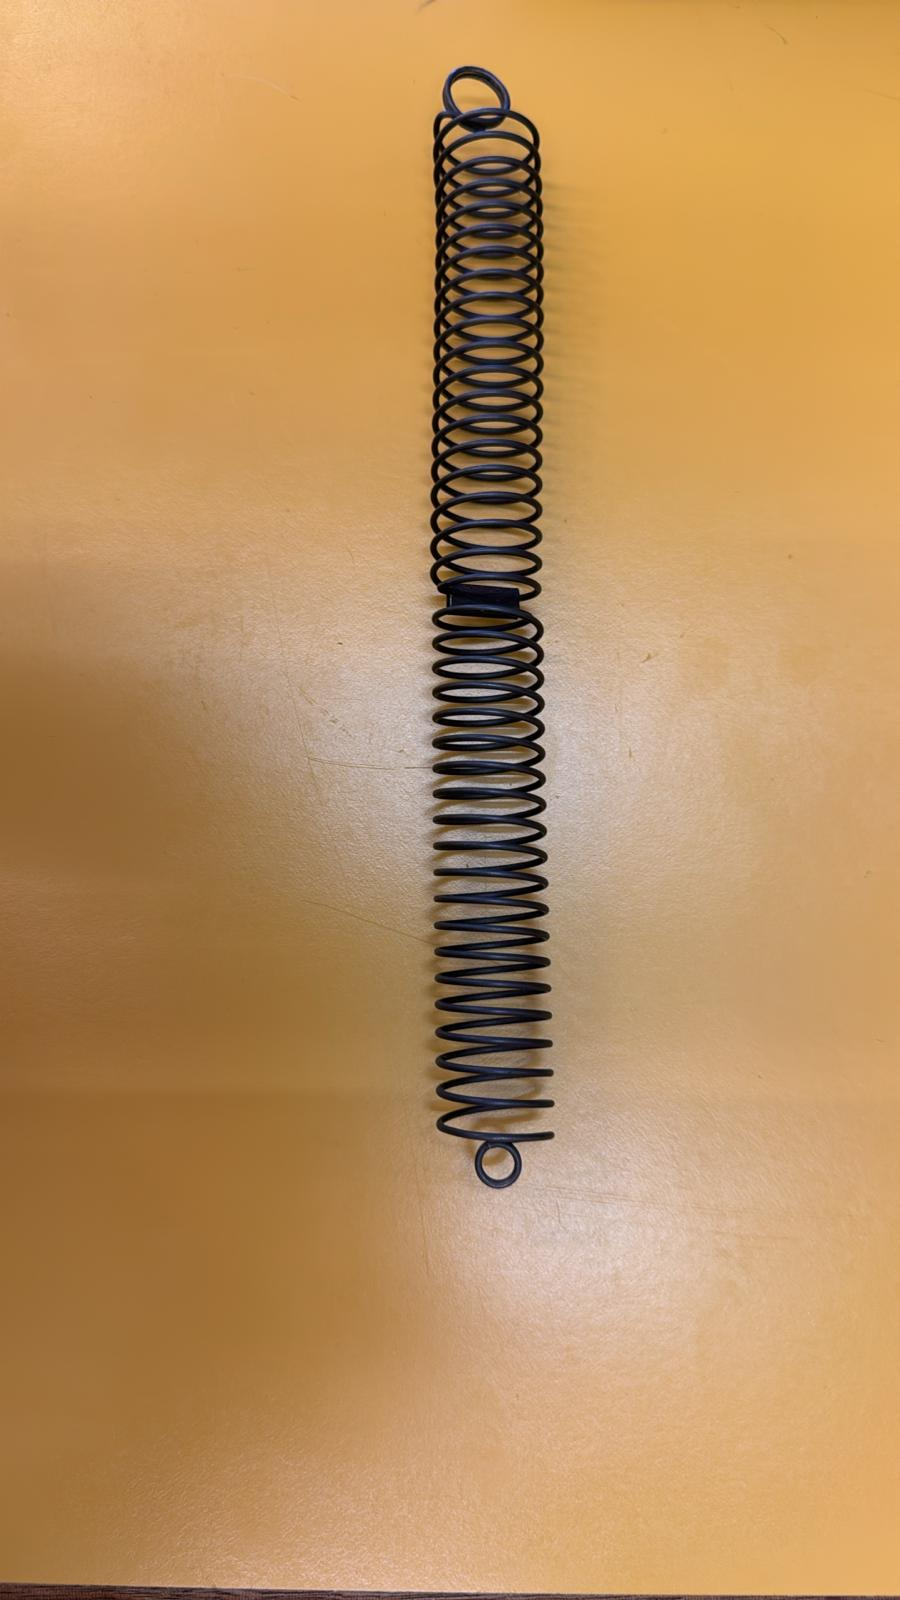
\includegraphics[width=0.77\linewidth]{images/res2.jpeg}
                    \caption{Ressort 1}
                \end{minipage}
                \hfill
                \begin{minipage}{0.32\textwidth}
                    \centering
                    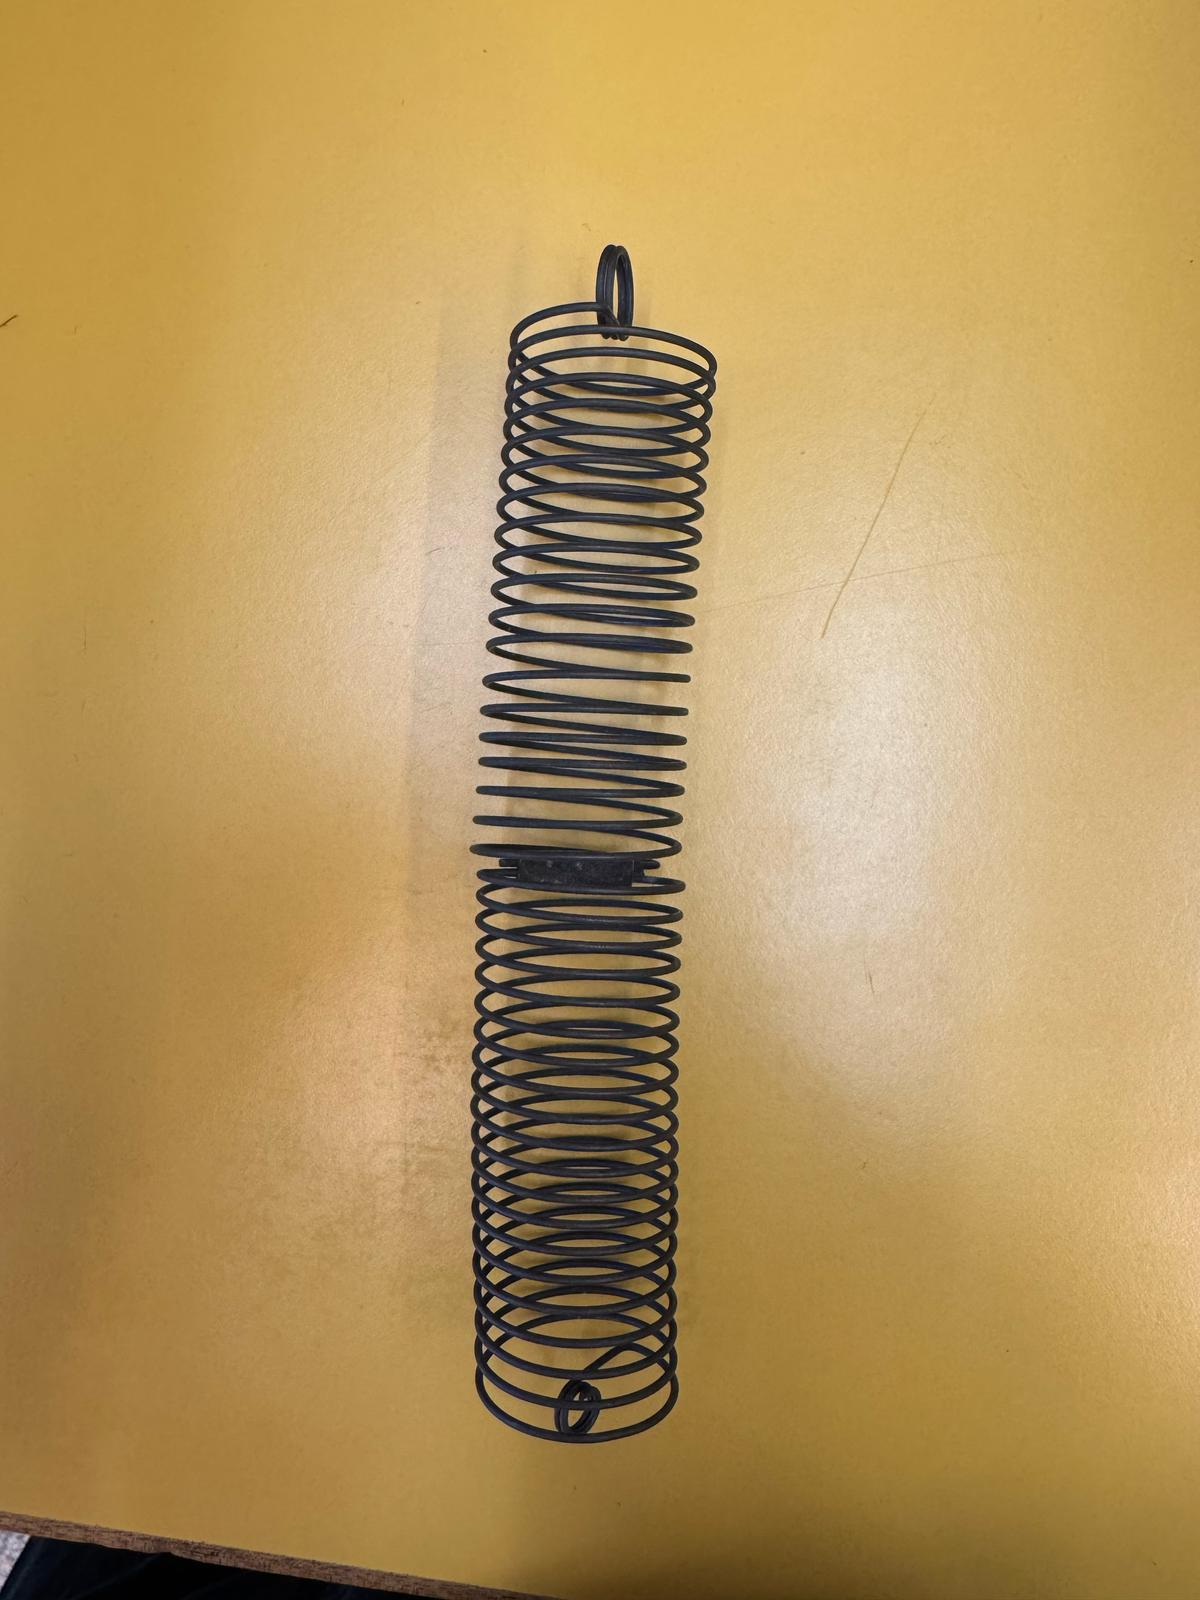
\includegraphics[width=\linewidth]{images/res1.jpeg}
                    \caption{Ressort 2}
                \end{minipage}
                \hfill
                \begin{minipage}{0.32\textwidth}
                    \centering
                    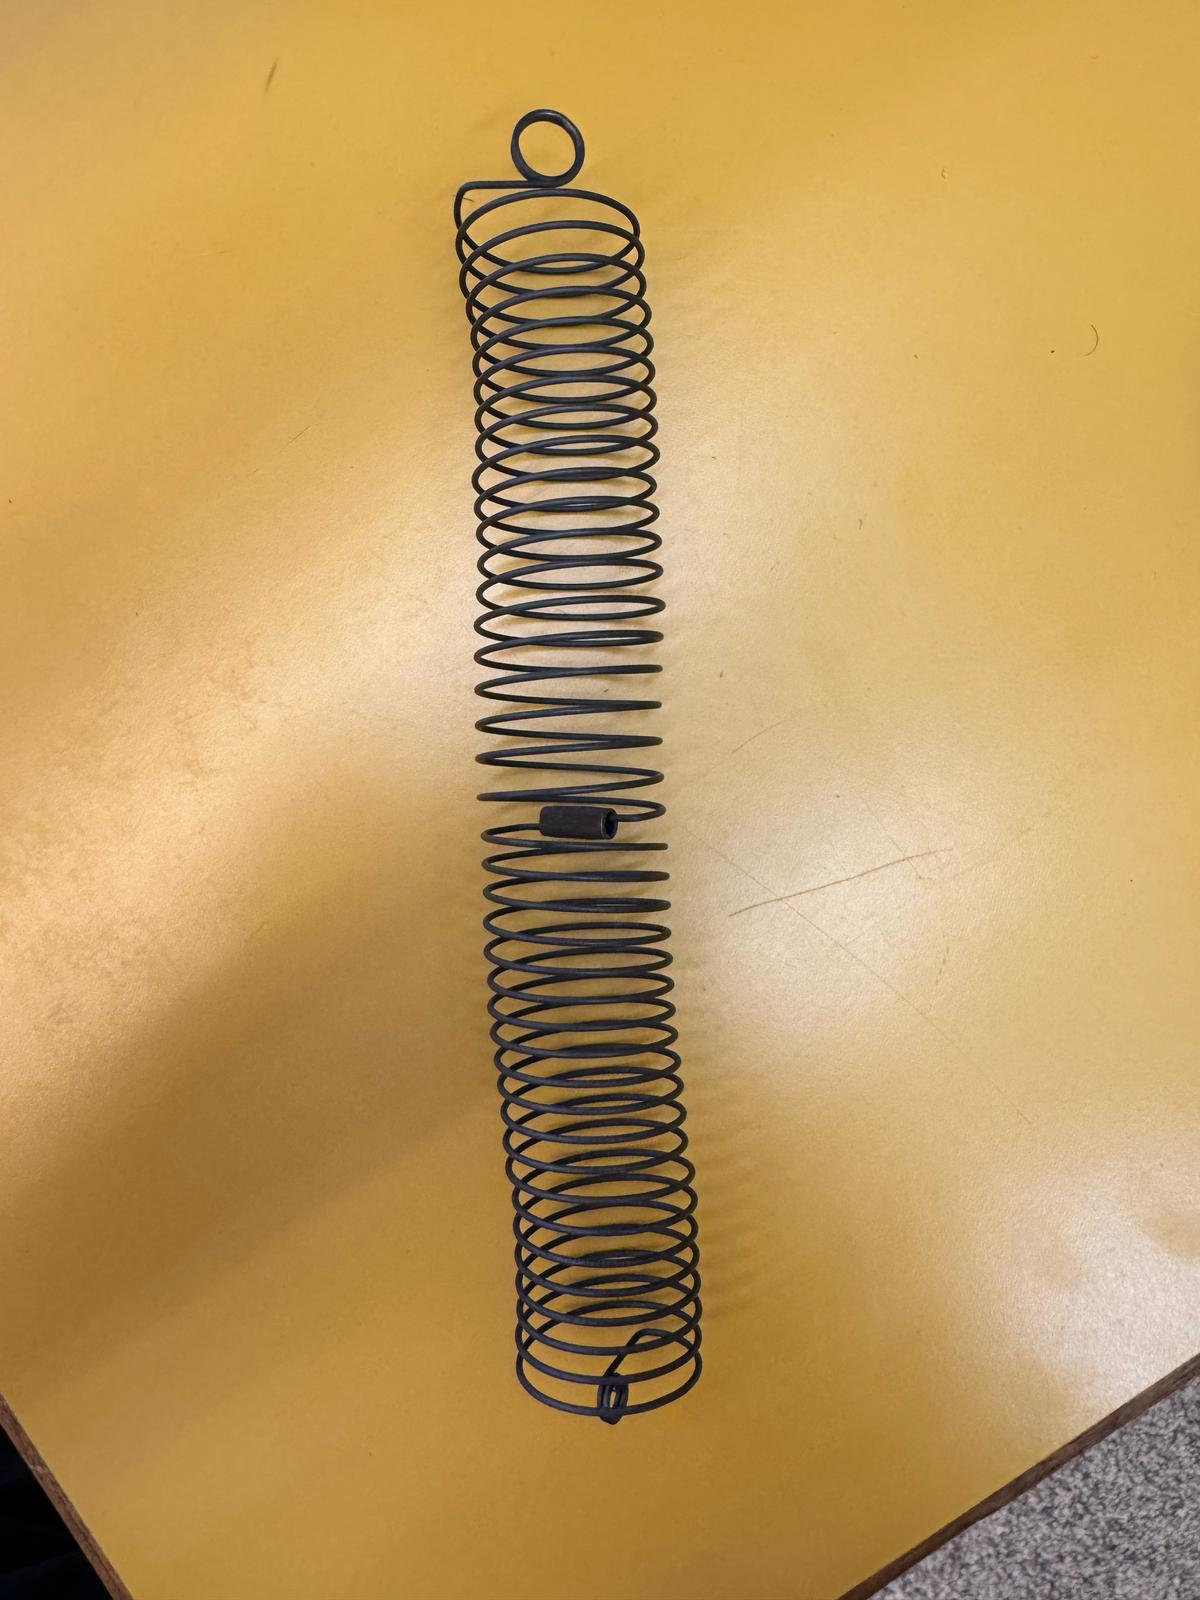
\includegraphics[width=\linewidth]{images/res3.jpeg}
                    \caption{Ressort 3}
                \end{minipage}
            \end{figure}
        \subsubsection{Discussion des résultats}
    \subsection{Détermination de la période d'un ressort}
        \subsubsection{Objectif}
        
        \subsubsection{schéma du système}
            \begin{figure}[h]
    \centering
    \begin{tikzpicture}
        % Equilibrium Position
        % Ground and frame
        \draw[thick] (-1,5) -- (1,5); % Top bar
        \draw[thick] (-1,5) -- (-1,0); % Side bar
        
        % Sensor
        \draw[fill, pattern=north east lines] (0.5,5) rectangle (1,5.5);
        
        % Laser
        \draw[red, thick] (0.75,5) -- (0.75,3.3); % Laser stopping at plate
        
        % Vertical x-axis with cut line (on the left)
        \node[below, blue] at (-1.2,0) {$x$};
        \draw[blue, thick, ->] (-1.2,5) -- (-1.2,0);
        \node[left, blue] at (-1.2,3.31) {$0$};
        \draw[blue, thick] (-1.25,3.31) -- (-1.15,3.31); % Cut mark for 0
        \draw[blue, thin] (-1.2,3.308) -- (-0.8,3.308); % Cut line from x-axis to plate
        
        % Spring (equilibrium position, more loops)
        \draw[decorate, decoration={coil,aspect=0.7,segment length=3.5mm,amplitude=3mm}] (0,5) -- (0,3.4);
        \draw[thin] (0,3.4) -- (0,3.3); % Extended bottom vertical line
        
        % Thin plate attached to the spring (longer and fully above mass)
        \draw[thick] (-0.8,3.3) rectangle (0.8,3.2); % Longer rectangle plate

    \end{tikzpicture}
    \hspace{1cm}
    \begin{tikzpicture}
        % Elongated Position
        % Ground and frame
        \draw[thick] (-1,5) -- (1,5); % Top bar
        \draw[thick] (-1,5) -- (-1,0); % Side bar
        
        % Sensor
        \draw[fill, pattern=north east lines] (0.5,5) rectangle (1,5.5);
        
        % Laser
        \draw[red, thick] (0.75,5) -- (0.75,1.8); % Laser stopping at plate
        
        % Vertical x-axis with cut line (on the left)
        \node[below, blue] at (-1.2,0) {$x$};
        \draw[blue, thick, ->] (-1.2,5) -- (-1.2,0);
        \node[left, blue] at (-1.2,1.8) {$x_1$};
        \draw[blue, thick] (-1.25,1.81) -- (-1.15,1.81); % Cut mark for X1
        \draw[blue, thin] (-1.2,1.81) -- (0,1.8); % Cut line from x-axis to plate
        
        % Spring (elongated position, more spaced loops, extended bottom part)
        \draw[decorate, decoration={coil,aspect=0.7,segment length=5mm,amplitude=3mm}] (0,5) -- (0,2.2);
        \draw[thick] (0,2.2) -- (0,1.8); % Extended bottom vertical line
        
        % Thin plate attached to the spring (longer and fully above mass)
        \draw[thick] (-0.8,1.8) rectangle (0.8,1.7); % Longer rectangle plate
        
        % Mass (elongated position, moved lower)
        \draw[thick] (-0.5,1.5) rectangle (0.5,1.0);
        \node at (0,1.25) {$m_s$};
        
        % Gravity
        \draw[->, teal, thick] (0,1.0) -- (0,0.3);
        \node[right, teal] at (0,0.2) {$m_s \vec{g}$};
        
        % Spring force
        \draw[->, teal, thick] (0,1.5) -- (0,2.3);
        \node[left, teal] at (0,2.3) {$\vec{F_r}$};
    \end{tikzpicture}
    \caption{Position au repos et position allongée du système à l'équilibre.}
\end{figure}
\FloatBarrier
            Nous remarquons que le schéma du système est le même que celui de l'expérience précédente.
            Nous avons donc le même dispositif, mais cette fois-ci, nous allons laisser le ressort
            osciller en lui donnant une amplitude initiale en l'étirant de $x_1$ (environ 1 à 2cm).

        \subsubsection{Notions théoriques}
            Pour pouvoir déterminer la période d'un ressort, nous devons tout d'abord poser les équations
            exprimée par la seconde loi de Newton. Nous avons donc :
            \begin{equation}
                \sum \vec{F}_{ext} = m \vec{a}
            \end{equation}
            Cette fois-ci, nous sommes en mouvement, donc nous avons une accélération non nulle.
            Nous pouvons poser la somme des forces comme suit :
            \begin{equation}
                \vec{F_r} + m_s\vec{g} = m_s \vec{a}
            \end{equation}
            \begin{align*}
                \Leftrightarrow & -kx \vec{e_x} + m_s g \vec{e_x} = m_s \ddot{x} \vec{e_x} \\
                \Leftrightarrow & -kx + m_s g = m_s \ddot{x} \\
                \Leftrightarrow & \ddot{x} + \frac{k}{m_s}x = g
            \end{align*}
            Nous avons une équation différentielle du second ordre, avec second membre non nul.
            Cependant, comme nous avons poser l'origine du repère à la position d'équilibre du ressort + surcharge,
            le terme $g$ disparaît. Nous avons donc une équation homogène du second ordre et ceci nous permet de
            déterminer la période du ressort. Nous avons donc :
            \begin{equation}
                \ddot{x} + \frac{k}{m_s}x = 0
            \end{equation}
            La forme standard de l'équation différentielle pour une oscillation harmonique simple est défini comme suit :
            \begin{equation}
                \ddot{x} + \omega^2 x = 0
            \end{equation}
            Où $\omega = \sqrt{\frac{k}{m_s}}$ est la pulsation propre du ressort.
            Nos conditions initiales sont $x(0) = x_1$ et $\dot{x}(0) = 0$.
            Nous avons donc la solution générale de l'équation différentielle :
            \begin{equation}
                x(t) = x_1 \cos(\omega t)
            \end{equation}
            Nous préferons sous forme d'une sinusoïde, donc nous avons :
            \begin{align*}
                x(t) = x_1 \cos(\omega t) = x_1 \sin(\omega t + \frac{\pi}{2})
            \end{align*}
            et ce qui nous donne :
            \begin{equation}
                x(t) = x_1 \sin(\omega t + \phi)
            \end{equation}
            où $\frac{\pi}{2}$ est absorbé par la phase $\phi$. \\
            Nous avons maintenant tout ce qu'il nous faut pour déterminer la période du ressort.
            Nous pouvons finalement poser que la période est donnée par :
            \begin{align*}
                \omega = \frac{2\pi}{T}
                \Leftrightarrow & T = \frac{2\pi}{\omega}
            \end{align*}
            et finalement :
            \begin{equation}
                T = 2\pi \sqrt{\frac{m_s}{k}}
            \end{equation}
            
            \newpage

            Il nous est demandé de déterminer l'incertitude sur la période du ressort.
            Nous savons que la formule pour détermination de l'incertitude d'une fonction quelconque de
            la forme $f(x, y, z, ...)$ est donnée par sa différentielle totale, avec des valeurs absolues pour
            chaque dérivée partielle, ce qui donne :
            \begin{equation}
                \Delta f(x, y, z, ...) = \left| \frac{\partial f}{\partial x} \right| \Delta x + \left| \frac{\partial f}{\partial y} \right| \Delta y + \left| \frac{\partial f}{\partial z} \right| \Delta z + ...
            \end{equation}
            Ici, la période est définie par $T(m_s, k) = 2\pi \sqrt{\frac{m_s}{k}}$, nous pouvons poser :
            \begin{align*}
                \Delta T = \left| \frac{\partial T}{\partial m_s} \right| \Delta m_s + \left| \frac{\partial T}{\partial k} \right| \Delta k
            \end{align*}
            ce qui nous donne :
            \begin{equation}
                \Delta T = \pi \frac{1}{\sqrt{m_s k}} \Delta m_s + \pi \frac{\sqrt{m_s}}{k^{3/2}} \Delta k
            \end{equation}

            
                    
    


    
    
        
